\chapter{Antecedentes y justificación}
\thispagestyle{fancy}
\fancyhead[LE]{\thechapter.Antecedentes y justificación}

\section{Antecedentes}
Este proyecto parte del proyecto de R.Sánchez\autocite{sanchez-corcueraPersuasionbasedRecommenderSystem2020} donde se desarrolló un sistema de recomendación de estrategias de persuasión basado en aprendizaje activo. Para comprender los antecedentes que han incurrido en el desarrollo de este proyecto primeró hay que conocer y comprender qué son los sistemas de recomendación y después entender los problemas de seguridad y privacidad que van ligados a estos. 
\subsection{Sistemas de recomendación}
Los sistemas de recomendación fueron mencionados por primera vez en los años 90 y han ido evolucionando hasta estar implantados en gran parte de las empresas actuales. Estos sistemas son sistemas de filtrado de información, que partiendo de una gran cantidad de datos, tanto del usuario como de los elementos a recomendar, pueden predecir cuál será el elemento más apropiado para el usuario. Estos sistemas están estrechamente relacionados con el marketing, ya que el objetivo es conseguir recomendar un elemento que sea del agrado e interés de los usuarios suele ir ligado a fines económicos.
\\ \\
Hoy en día se usan en multitud de ámbitos, desde las redes sociales hasta las distribuidoras de contenido como Netflix, pasando por compañías de comercio electrónico como Amazon. 
\\ \\
A la hora de realizar la recomendación se realizan filtrados de diferente tipo, estos no son más que la forma en la que el sistema busca correlacionar los usuarios con los elementos que estos consumen, compran o ven. Entre los métodos más comunes para relacionar esta información y obtener resultados eficientes se encuentran:
\begin{itemize}
    \item Filtros demográficos, que recomiendan en función del sexo, edad, país, oficio,… 
    \item Filtros basados en contenidos, como Youtube, que recomiendan contenidos similares a los valorados por los usuarios. 
    \item Filtrado colaborativo, que consiste en recomendar al usuario elementos valorados positivamente por usuarios similares a él. 
\end{itemize}

Sin embargo, existen sistemas híbridos que utilizan varias de las estrategias de filtrado anteriores combinadas. Un ejemplo de ello es el mencionado Amazon, que tiene uno de los algoritmos de recomendación más potentes y eficientes actualmente. 
\\ \\
Sin embargo, existen sistemas híbridos que utilizan varias de las estrategias de filtrado anteriores combinadas. Un ejemplo de ello es el mencionado Amazon, que tiene uno de los algoritmos de recomendación más potentes y eficientes actualmente. 
\\ \\
Esto se debe a dos cosas, en primer lugar que cuenta con una gran cantidad de información de los usuarios, tanto su edad, género, país, dirección, rutinas (si tienen Alexa), … como los artículos que miran, compran, añaden a la lista, etc. Con todo esto el algoritmo es capaz de ofrecer recomendaciones muy precisas a los usuarios, lo que le da una gran calidad de servicio a la empresa gracias a esto.
\\ \\
De hecho, en Amazon, si queremos revisar las recomendaciones tenemos un apartado propio para ellas al que se puede acceder fácilmente (Fig\ref{fig:AmazonRecomendaciones}).
\begin{figure}[thbp]
    \centering
    \fbox{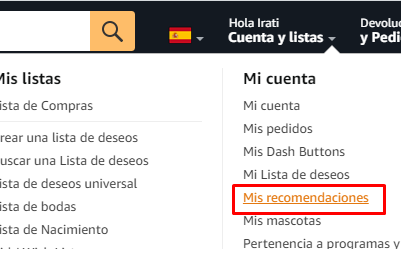
\includegraphics[width=0.45\textwidth]{Figuras/Amazon_acceder_mis_recomendaciones.png}}
    \fbox{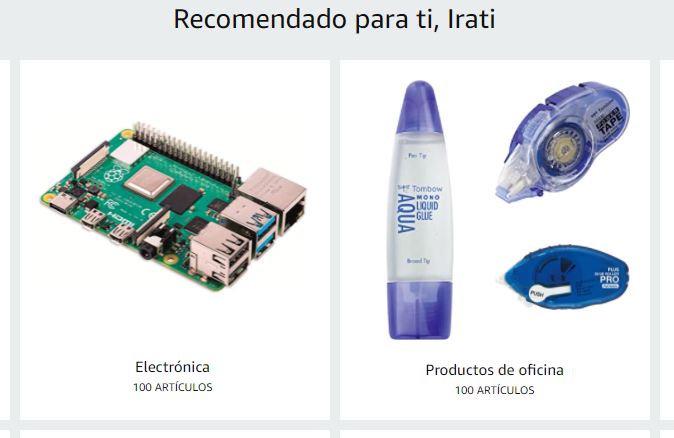
\includegraphics[width=0.45\textwidth]{Figuras/Amazon_recomendaciones.png}}
    \caption{Recomendaciones de Amazon (Fuente: Amazon\autocite{AmazonEsCompra})} 
    \label{fig:AmazonRecomendaciones}
\end{figure}

\subsection{Privacidad digital}
Queda claro que un sistema de recomendación depende plenamente de la información de la que dispone, de forma que, de cuanta más información disponga de los usuarios, más precisión tendrá en sus predicciones. Para obtener esta información muchos anunciantes se han valido de diversas herramientas y utilidades, pero si se ha de destacar alguna son las cookies de terceros. Estas, son definidas por Google\autocite{ComoBorrarHabilitar} cómo:
\\
\begin{minipage}[t]{0.2\linewidth}
\end{minipage}
\hfill
\begin{minipage}[t]{0.9\linewidth}
  \textit{"... son archivos que crean los sitios web que visitas para guardar información de la navegación y facilitar tu experiencia en línea. Gracias a las cookies, los sitios pueden mantener abierta tu sesión, recordar tus preferencias del sitio y proporcionarte contenido relevante en función del lugar donde te encuentres. Hay dos tipos de cookies:
  \begin{itemize}
      \item Las cookies de origen, que las crea el sitio que visitas. El sitio se muestra en la barra de direcciones.
      \item Las cookies de terceros, que las crean otros sitios. Parte del contenido que ves en la página web que visitas, como anuncios o imágenes, pertenece a estos sitios."
  \end{itemize}}
\end{minipage}
\\ \\
A simple vista estas cookies parecen inofensivas, pero el problema radica en su utilización. Aunque suelen ser usadas con fines analíticos por compañías de marketing online, estas se usan para registrar el comportamiento de un usuario y crear un perfil para generar publicidad personalizada. Mediante estas se puede registrar el comportamiento de un usuario en internet, saber sus movimientos, hábitos, páginas que visita, edad, sexo, etc. 
\\ \\
En España y en la Unión Europea existe una legislación sobre la privacidad y la protección de datos que restringe y limita los datos que estas empresas pueden registrar de nuestra navegación, el Reglamento General De Protección de Datos (RGPD). En el documento adjunto Anexo \ref{appendix:ProteccionDatos}, sección \ref{appendix:ProteccionDatos_Legislacion} se puede consultar un breve resumen de la legislación en vigor. En lo referente a las cookies este reglamento presenta varios elementos importantes. En primer lugar, debe haber un consentimiento explicito por el usuario en el consentimiento de la política de cookies. En segundo lugar, la aceptación de las cookies de terceros no ha de ser un impedimento para el uso del servicio. En último lugar, todas las cookies y rastreadores que operen en la web del propietario deberán ser mostradas al usuario en un lenguaje sencillo.
\\ \\
De todos modos esta legislación no impide que se realice un perfilado del usuario, que se haga un seguimiento de este por la red o que se analice el tiempo que pasa el usuario en la página. Pero con la maduración de la tecnología cada vez más gente se preocupa por el uso que le dan estas empresas a los datos y son más críticos con estas prácticas. Esto ha llegado incluso a la política, donde España esta desarrollando una carta pionera de derechos digitales, donde, entre otras cosas, recoge el derecho de los usuarios a no ser perfilados (Anexo \ref{appendix:ProteccionDatos}, sección \ref{appendix:ProteccionDatos_Derechos}).
\\ \\
Hoy en día existen muchos navegadores y complementos que permiten bloquear este tipo de rastreadores, lo que ha llevado al sector y a Google a tener que explorar nuevas vías para obtener esta información. La solución propuesta por Google ha sido su nuevo sistema Federated Learning of Cohorts, aprendizaje federado de cortes, con el que se compromete a dejar las cookies de terceros.
\\ \\
Lo que a priori puede significar una buena noticia no es para nada la realidad. Este sistema permite a Google y a su navegador agrupar usuarios en base a sus intereses y perfiles geográficos gracias al historial de navegación y a los datos recogidos durante la navegación. Aunque permite que los usuarios no puedan ser distinguidos dentro de un grupo este perfilado supone una persecución y rastreo más grave que la acaecida por las cookies de terceros. En primer lugar, sitúa a Google como principal proveedor de marketing digital, lo que afectaría tanto a las funciones que podrían desempeñar las empresas de marketing digital como al precio que tendrían que pagar por la información.
\\ \\
Ante esta imposición de Google varias empresas se han pronunciado y han expresado su total desacuerdo con la política, navegadores como DuckDuckGo o Brave la han calificado de anticompetitiva, invasiva y abusiva. Esto se debe a que el navegador de Google, Google Chrome, acapara el 64.19\%\footnote{Fuente: https://gs.statcounter.com/, 27/04/2021} de la red y podría obligar a utilizar su sistema a muchos anunciantes y sitios web.
\\ \\  
Cabe destacar que este sistema aun no ha sido aprobado por la Unión Europea, para ello se debe comprobar que cumpla el RGPD y no vulnere ningún derecho de los ciudadanos.

\section{Justificación}
Este proyecto es una respuesta a todo lo anterior,al estado de la industria del marketing digital, donde se exprimen al máximo las leyes y normas sobre protección de datos y privacidad digital, y a la actitud de las grandes empresas por perfilar a los usuarios y recoger tanta información de estos como les sea posible. Se quiere demostrar que se puede utilizar el aprendizaje federado preservando la privacidad de los usuarios en un sistema de recomendación, permitiéndoles tener el control total sobre su información en su propio dispositivo. 
\\ \\
Además, para ello se utilizarán dispositivos como las Raspberry Pis, las cuales servirán para demostrar que no se necesitan dispositivos especialmente potentes para participar en una red de aprendizaje federado. Evidenciando que es posible implementar un sistema de recomendación respetuoso con el usuario, acorde al RGPD y salvaguardando los derechos digitales.
